\documentclass[12pt, dvipdfmx]{beamer}

\renewcommand{\kanjifamilydefault}{\gtdefault}
%%%%%%%%%%%  package  %%%%%%%%%%%
\usepackage{bxdpx-beamer}% dvipdfmxなので必要
\usepackage{pxjahyper}% 日本語で'しおり'したい

\usepackage{amssymb,amsmath,ascmac}

\usepackage{multirow}
\usepackage{bm}

\graphicspath{{../Figures/simulation}}

\usepackage{tikz}
\usepackage{xparse}

\usepackage{multimedia}

\usetikzlibrary{shapes,arrows}
%% define fancy arrow. \tikzfancyarrow[<option>]{<text>}. ex: \tikzfancyarrow[fill=red!5]{hoge}
\tikzset{arrowstyle/.style n args={2}{inner ysep=0.1ex, inner xsep=0.5em, minimum height=2em, draw=#2, fill=black!20, font=\sffamily\bfseries, single arrow, single arrow head extend=0.4em, #1,}}
\NewDocumentCommand{\tikzfancyarrow}{O{fill=black!20} O{none}  m}{
\tikz[baseline=-0.5ex]\node [arrowstyle={#1}{#2}] {#3 \mathstrut};}

%微分関連のマクロ
%
\newcommand{\diff}{\mathrm d}
\newcommand{\difd}[2]{\dfrac{\diff #1}{\diff #2}}
\newcommand{\difp}[2]{\dfrac{\partial #1}{\partial #2}}
\newcommand{\difdd}[2]{\dfrac{\diff^2 #1}{\diff #2^2}}
\newcommand{\difpp}[2]{\dfrac{\partial^2 #1}{\partial #2^2}}

%目次スライド
% \AtBeginSection[]{
%   \frame{\tableofcontents[currentsection]}
% }

%アペンディックスのページ番号除去
\newcommand{\backupbegin}{
   \newcounter{framenumberappendix}
   \setcounter{framenumberappendix}{\value{framenumber}}
}
\newcommand{\backupend}{
   \addtocounter{framenumberappendix}{-\value{framenumber}}
   \addtocounter{framenumber}{\value{framenumberappendix}} 
}

\newcommand{\rmd}{\mathrm{d}}
\newcommand{\dd}[1]{\dfrac{\mathrm{d} #1}{\mathrm{d} x}}

%%%%%%%%%%%  theme  %%%%%%%%%%%
\usetheme{Copenhagen}
% \usetheme{Metropolis}
% \usetheme{CambridgeUS}
% \usetheme{Berlin}

%%%%%%%%%%%  inner theme  %%%%%%%%%%%
% \useinnertheme{default}

% %%%%%%%%%%%  outer theme  %%%%%%%%%%%
\useoutertheme{default}
% \useoutertheme{infolines}

%%%%%%%%%%%  color theme  %%%%%%%%%%%
%\usecolortheme{structure}

%%%%%%%%%%%  font theme  %%%%%%%%%%%
\usefonttheme{professionalfonts}
%\usefonttheme{default}

%%%%%%%%%%%  degree of transparency  %%%%%%%%%%%
%\setbeamercovered{transparent=30}

% \setbeamertemplate{items}[default]

%%%%%%%%%%%  numbering  %%%%%%%%%%%
% \setbeamertemplate{numbered}
\setbeamertemplate{navigation symbols}{}
\setbeamertemplate{footline}[frame number]

%%%%%%%%%%%%%%%%%%%%%%%%%%%%%%%%%%%
\title
{接着部材への水の浸透}
\subtitle{基材近傍での拡散挙動}
\author[東亞合成 佐々木]{佐々木裕}
\institute[東亞合成]{東亞合成}
\date{October 29, 2021}
%%%%%%%%%%%%%%%%%%%%%%%%%%%%%%%%%%
\begin{document}
%%%%%%%%%%%%%%%%%%%%%%%%%%%%%%%%%%
\begin{frame}\frametitle{}
	\titlepage
\end{frame}
% %%%%%%%%%%%%%%%%%%%%%
% \section*{}
% %
% \begin{frame}
% %[allowframebreaks]
% {Outline}
% 	\tableofcontents
% \end{frame}

%%%%%%%%%%%%%%%%%%%%%
\section{やりたいこと}
%%%%%%%%%%%%%%%%%%%%%%%%%%%%%%%%%%%%%%%%%%%%%
\subsection{説明}

\begin{frame}
	\frametitle{接着基材と水}
        \begin{block}{接着状態への水の影響}
            \begin{itemize}
                \item 接着端部からの水の拡散
                \item 接着不良の大きな原因
            \end{itemize}
        \end{block}
        
				\begin{center}
					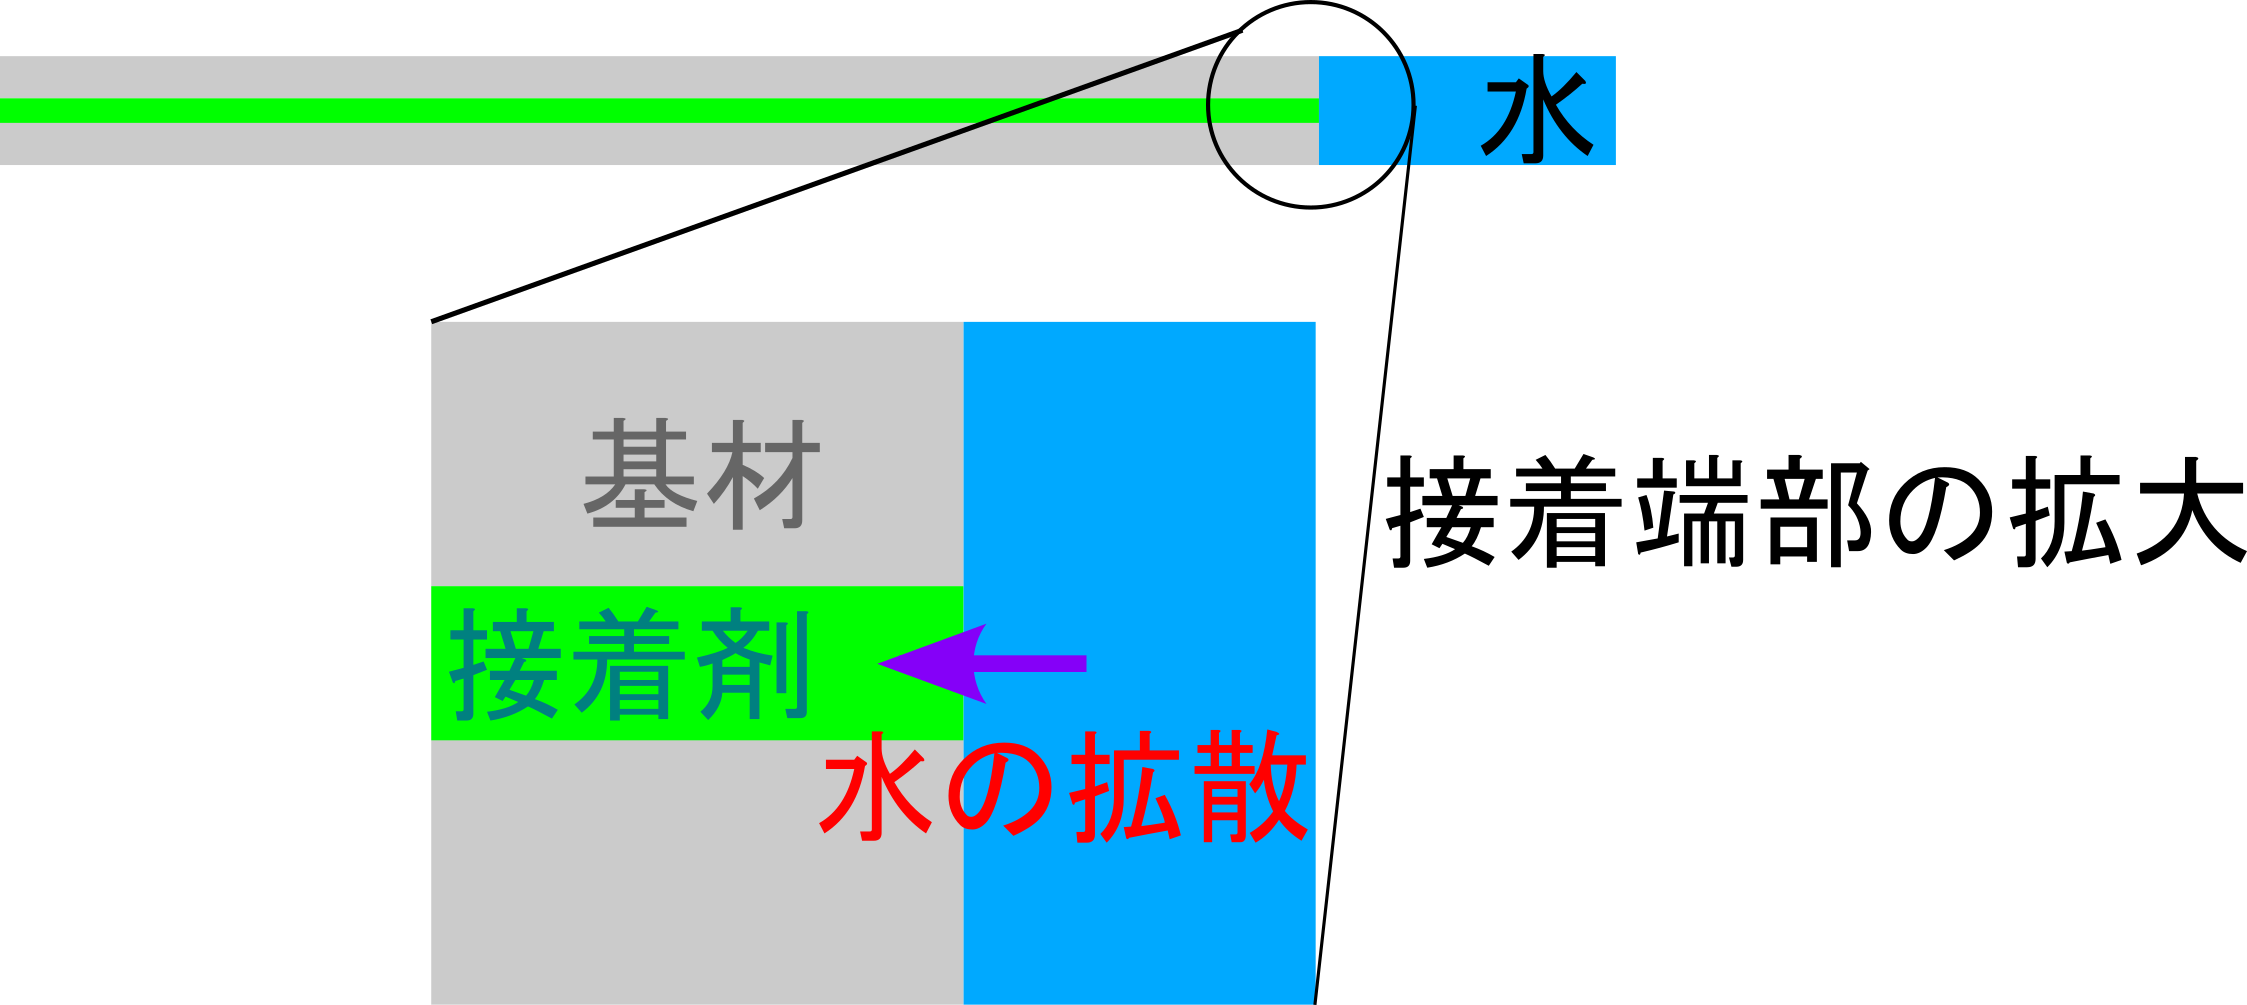
\includegraphics[width=.9\textwidth]{adherent_water.png}
				\end{center}
\end{frame}

\begin{frame}
	\frametitle{基材との界面近傍での振る舞い}
        \begin{block}{水の影響}
            \begin{itemize}
                \item 実験での現象
                \begin{itemize}
                    \item バルクでの拡散速度から予測される浸透時間よりも\\短い時間での界面破壊
                \end{itemize}
                \item 低分子物質の界面での一般的な振る舞い
                \begin{itemize}
                    \item 形態エントロピーのロスの少ない低分子物質が\\界面近傍へ偏析
                \end{itemize}
            \end{itemize}
        \end{block}
        
				\begin{center}
					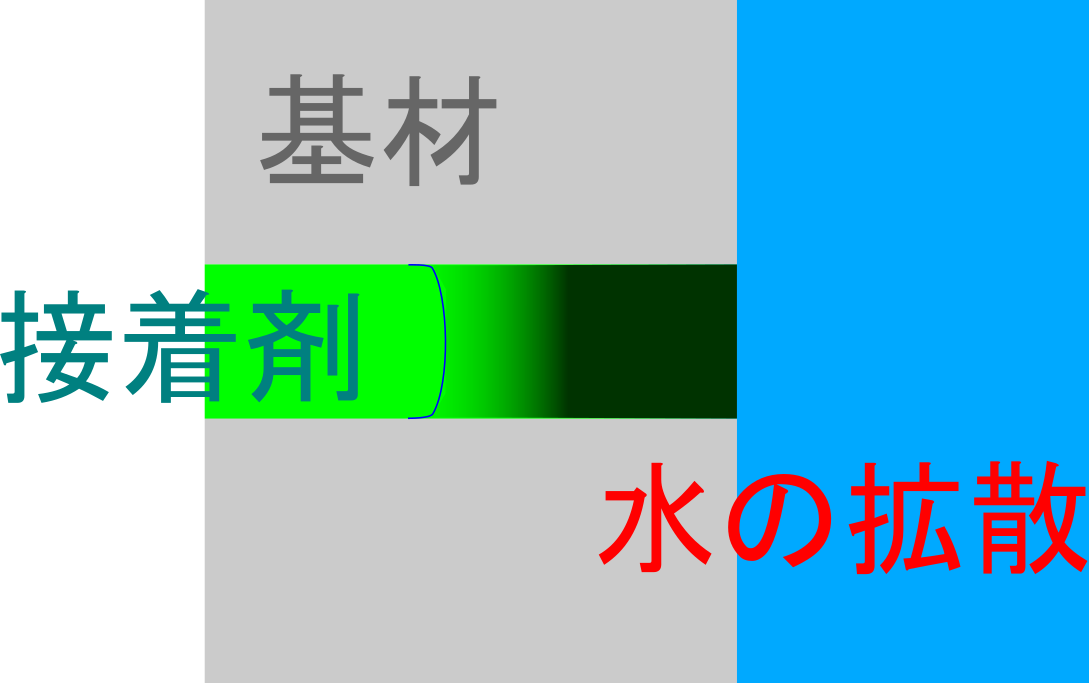
\includegraphics[width=.5\textwidth]{adherent_water_2.png}
				\end{center}
\end{frame}
\end{document}
